\documentclass[11pt]{article}
\usepackage{booktabs}
\usepackage{natbib}
\usepackage{fullpage}
\usepackage{fancyhdr}
\usepackage{rotating}

\usepackage{amsmath}
\usepackage{amssymb}
\usepackage{url}

\usepackage{listings}
\usepackage{color}
\lstset{%
        basicstyle=\footnotesize\ttfamily,
        showspaces=false,
        showstringspaces=false,
        tabsize=2,
        breaklines=false,
        breakatwhitespace=true,
        identifierstyle=\ttfamily,
        keywordstyle=\color[rgb]{0,0,1},
        commentstyle=\color[rgb]{0.133,0.545,0.133},
        stringstyle=\color[rgb]{0.627,0.126,0.941},
    }

\usepackage{graphicx}

% header
\fancyhead{}
\fancyfoot{}
\fancyfoot[C]{\thepage}
\fancyhead[R]{Daniel Foreman-Mackey}
\fancyhead[L]{Statistical Natural Language Processing --- Final Project}
\pagestyle{fancy}
\setlength{\headsep}{10pt}
\setlength{\headheight}{20pt}

% shortcuts
\newcommand{\Eq}[1]{Equation (\ref{eq:#1})}
\newcommand{\eq}[1]{Equation (\ref{eq:#1})}
\newcommand{\eqlabel}[1]{\label{eq:#1}}
\newcommand{\Fig}[1]{Figure~\ref{fig:#1}}
\newcommand{\fig}[1]{Figure~\ref{fig:#1}}
\newcommand{\figlabel}[1]{\label{fig:#1}}

\newcommand{\etal}{\emph{et al.}}

\newcommand{\pr}[1]{\ensuremath{p\left (#1 \right )}}
\newcommand{\lk}[1]{\ensuremath{\mathcal{L} \left ( #1 \right )}}
\newcommand{\bvec}[1]{\ensuremath{\boldsymbol{#1}}}
\newcommand{\dd}{\ensuremath{\, \mathrm{d}}}
\newcommand{\normal}[2]{\ensuremath{\mathcal{N} \left ( #1; #2 \right ) }}
\newcommand{\T}{^\mathrm{T}}
\newcommand{\expect}[2]{\ensuremath{\mathrm{E}_{#1}\left [ {#2} \right ]}}

\newcommand{\data}{\mathcal{D}}
\newcommand{\code}[1]{{\sffamily #1}}
\DeclareMathOperator*{\argmax}{arg\,max}
\DeclareMathOperator*{\argmin}{arg\,min}


\begin{document}

\section{Variational LDA}

Th basic LDA model is shown in the top panel of \fig{lda}.
In this model, there is a set of $K$ topics that describe $D$ documents with
$N_d$ words (in a vocabulary of $J$ words) each.
The generative procedure is:
\begin{itemize}
\item{for each topic $k=1,\cdots,K$, draw a word distribution
$\beta_k \sim \mathrm{Dirichlet}(\eta)$,}
\item{for each document $d=1,\cdots,D$, draw a topic distribution $\theta_d
\sim \mathrm{Dirichlet}(\alpha)$, and then}
\item{for each word $n=1,\cdots,N_d$, draw a topic
$z_{d,n}\sim\mathrm{Multinomial}(\theta_d)$ and specific word
$w_{d,n}\sim\mathrm{Multinomial}(\beta_{z_{d,n}})$.}
\end{itemize}
To be specific, the relevant distributions are
\begin{eqnarray}
p(\beta_k\,|\,\eta) &=&
\frac{\Gamma\left( \sum_j \eta_j \right)}{\sum_j \Gamma(\eta_j)} \,
\prod_{j=1}^J \beta_{k,j}^{\eta_j-1} \quad, \\
p(\theta_d\,|\,\alpha) &=&
\frac{\Gamma\left( \sum_k \alpha_k \right)}{\sum_k \Gamma(\alpha_k)} \,
\prod_{k=1}^K \theta_{d,k}^{\alpha_k-1} \quad, \\
p(z_{d,n}\,|\,\theta_d) &=& \theta_{d,z_{d,n}} \quad, \\
p(w_{d,n}\,|\,z_{d,n},\beta) &=& \beta_{z_{d,n},w_{d,n}} \quad.
\end{eqnarray}

To do parameter estimation in this model, we need to compute the marginalized
likelihood
\begin{eqnarray}
p(w\,|\,\alpha,\eta) &=& \int\dd\beta\dd\theta\dd z \,
    p(w,z,\theta,\beta\,|\,\alpha,\eta)
\end{eqnarray}
and optimize but this marginalization is intractable so we have to resort to
approximate methods.
Following \citet{lda}, we'll describe the mean field variational approach.
In this framework, an approximate model is postulated and the inference
becomes an optimization of the KL divergence.
The bottom panel of \fig{lda} shows the commonly used mean field model.
The approximate distributions are:
\begin{eqnarray}
q(\beta_k\,|\,\lambda_k) &=&
\frac{\Gamma\left( \sum_j \lambda_{k,j} \right)}{\sum_j \Gamma(\lambda_{k,j})}
\, \prod_{j=1}^J \beta_{k,j}^{\lambda_{k,j}-1} \quad, \\
q(\theta_d\,|\,\gamma_d) &=&
\frac{\Gamma\left( \sum_j \gamma_{d,j} \right)}{\sum_j \Gamma(\gamma_{d,j})}
\, \prod_{j=1}^J \theta_{d,j}^{\gamma_{d,j}-1} \quad, \\
q(z_{d,n}\,|\,\phi_{d,n}) &=& \phi_{d,n} \quad.
\end{eqnarray}
Given this approximate distribution, the inference problem is solved by
performing the optimization
\begin{eqnarray}\eqlabel{opt}
(\lambda^*,\,\gamma^*,\,\phi^*) &=& \argmax_{\lambda,\gamma,\phi}
\,\mathrm{D}\left [ q(\beta,\theta,z\,|\,\lambda,\gamma,\phi)\,||\,
p(\beta,\theta,z\,|\,w,\eta,\alpha)\right ]
\end{eqnarray}
where D is the KL divergence.
These optimal parameters then provide approximate posterior distributions for
$\beta$, $\theta$, and $z$.

The optimization in \eq{opt} can be rewritten---using Jensen's inequality---as
a maximization of the ``evidence lower bound'' (ELBO)
\begin{eqnarray}
\mathcal{L}(w,\lambda,\gamma,\phi) &=&
\expect{q}{\log p(w,\beta,\theta,z\,|\,\eta,\alpha)}
- \expect{q}{\log q(\beta,\theta,z\,|\,\lambda,\gamma,\phi)} \\
&\le& \log p(w\,|\,\alpha,\eta) \quad.
\end{eqnarray}
Using the fact that the model factorizes as shown in \fig{lda}, the ELBO can
be rewritten as
\begin{eqnarray}
\mathcal{L}(w,\lambda,\gamma,\phi) &=&
    \sum_{d=1}^D\left \{ \frac{1}{D}\,\sum_{k=1}^K \left (
    \expect{q}{\log p(\beta_k\,|\,\eta)}
    -\expect{q}{\log q(\beta_k\,|\,\lambda_k)} \right )\right.
\nonumber\\ &&
    +\sum_{n=1}^{N_d} \left ( \expect{q}{\log p(z_{d,n}\,|\,\theta_d)}
    +\expect{q}{\log p(w_{d,n}\,|\,z_{d,n},\beta)}
    -\expect{q}{\log q(z_{d,n}\,|\,\phi_{d,n})} \right)
\nonumber\\ &&  \left.
    +\expect{q}{\log p(\theta_d\,|\,\alpha)}
    -\expect{q}{\log q(\theta_d\,|\,\gamma_d)}
\right \} \\
&\equiv& \sum_d \ell_d (w,\lambda,\gamma_d,\phi_d) \quad.
\end{eqnarray}
Using the explicit distributions listed above and using constant $\eta_j =
\eta$ and $\alpha_k = \alpha$, the per-document term can be rewritten as
\begin{eqnarray}
\ell_d (w,\lambda,\gamma_d,\phi_d) &=&
[\log\Gamma(J\,\eta)-J\,\log\Gamma(\eta)]/D +
\log\Gamma(K\,\alpha)-K\,\log\Gamma(\alpha)
\nonumber \\
&& +\sum_k\log\Gamma(\gamma_{d,k}) -
\log\Gamma\left(\sum_k \gamma_{d,k}\right)
\nonumber\\
&& +\sum_{k=1}^K\left\{\frac{1}{D}\sum_j \log\Gamma(\lambda_j) -
\frac{1}{D}\log\Gamma\left(\sum_j \lambda_j\right)
\right. \nonumber\\
&& \quad+\sum_{n=1}^{N_d} \phi_{d,n,k}\,\left(
\expect{q}{\log\theta_{d,k}} + \expect{q}{\log\beta_{k,w_{d,n}}}
-\log\phi_{d,n,k}
\right)
\nonumber\\
&& \quad+ (\alpha-\gamma_{d,k})\,\expect{q}{\log\theta_{d,k}} +
\left.\sum_{j=1}^J (\eta-\lambda_{k,j})\,\expect{q}{\log\beta_{k,j}}
\right\} \quad.
\end{eqnarray}

Taking the gradient of this term and setting it to zero, we can find the
variational update equations
\begin{eqnarray}
\phi_{d,n,k} &\gets& \frac{1}{Z} \exp \left(\expect{q}{\log\theta_{d,k}}
+\expect{q}{\log\beta_{k,n}}\right) \\
\gamma_{d,k} &\gets& \alpha + \sum_n^{N_d} \phi_{d,n,k} \\
\lambda_{k,n} &\gets& \eta + \sum_{d=1}^{D} \phi_{d,n,k} \quad.
\end{eqnarray}

Finally, the expectations of the latent variables under the variational
distribution are
\begin{eqnarray}
\expect{q}{\log\theta_{d,k}} &=& \Psi(\gamma_{d,k})
    - \Psi\left(\sum_k \gamma_{d,k}\right) \\
\expect{q}{\log\beta_{k,n}} &=& \Psi(\lambda_{k,n})
    - \Psi\left(\sum_n \gamma_{k,n}\right)
\end{eqnarray}
where $\Psi$ is the derivative of the logarithm of the gamma function.

\begin{figure}
\begin{center}
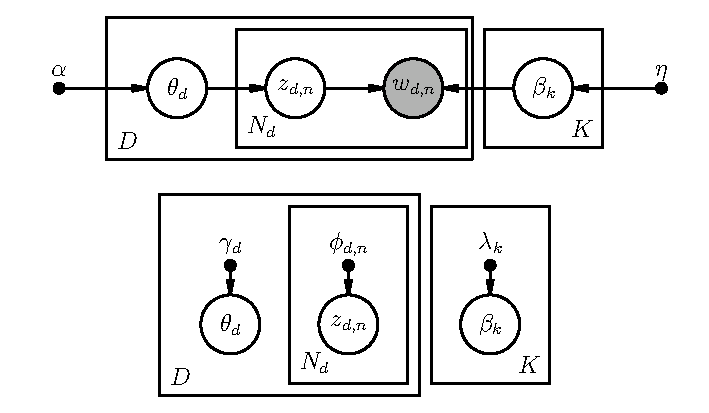
\includegraphics{lda.pdf}
\end{center}
\caption{%
LDA
\figlabel{lda}}
\end{figure}

\begin{thebibliography}{}\raggedright

\bibitem[Blei, Ng \& Jordan(2003)]{lda}
D. Blei, A. Ng, \& M. Jordan. \textbf{Latent Dirichlet allocation}.
\emph{Journal of Machine Learning Research}, 3:993–1022, January 2003.

\end{thebibliography}

\appendix

\section{Derivations of Variational Expectations}

For simplicity, we'll assume that the hyperparameters $\alpha$ and $\eta$ are
constant
\begin{eqnarray}
\alpha_k = \alpha\quad\forall k &\mathrm{and}&
\eta_j = \eta\quad\forall j \quad.
\end{eqnarray}

\begin{eqnarray}
\expect{q}{\log p(\beta_k\,|\,\eta)} &=&
\log \Gamma (J\,\eta) - \log \left ( J\,\Gamma(\eta) \right )
+ (\eta-1)\,\sum_{j=1}^J \expect{q}{\log\beta_{k,j}} \nonumber\\
&=&
\log \Gamma (J\,\eta) - \log \left ( J\,\Gamma(\eta) \right )
+ (\eta-1)\,\sum_{j=1}^J \left[ \Psi (\lambda_{k,j})
- \Psi({\textstyle\sum}_{j=1}^J \lambda_{k,j}) \right] \quad.
\end{eqnarray}
A similar expression holds for $\expect{q}{\log p(\theta_d\,|\,\alpha)}$.

For the document level expectations,
\begin{eqnarray}
\expect{q}{\log p(z_{d,n}\,|\,\theta_d)} &=&
\sum_{k=1}^K
\expect{q}{\log \theta_{d,k}} \nonumber \\
&=&
\sum_{k=1}^K
\phi_{d,n,k}
\left[\Psi (\gamma_{n,k}) - \Psi({\textstyle\sum}_{k^\prime=1}^K
\gamma_{n,k^\prime})
\right]
\end{eqnarray}
and
\begin{eqnarray}
\expect{q}{\log p(w_{d,n}\,|\,z_{d,n},\beta)} &=&
\sum_{k=1}^K
\expect{q}{\log \beta_{k,w_{d,n}}} \nonumber\\
&=&
\sum_{k=1}^K
\phi_{d,n,k}
\left[
\Psi (\lambda_{k,w_{d,n}})
- \Psi({\textstyle\sum}_{k^\prime=1}^K \lambda_{k^\prime,w_{d,n}})
\right] \quad.
\end{eqnarray}

Finally, for the expectations of the variational distributions,
\begin{eqnarray}
\expect{q}{\log q(\beta_k\,|\,\lambda_k)} &=&
\log \Gamma (\sum_k\lambda_k) - \log \left ( \sum_k\,\Gamma(\lambda_k) \right )
+ (\eta-1)\,\sum_{j=1}^J \expect{q}{\log\beta_{k,j}} \nonumber\\
&=&
\log \Gamma (J\,\eta) - \log \left ( J\,\Gamma(\eta) \right )
+ (\eta-1)\,\sum_{j=1}^J \left[ \Psi (\lambda_{k,j})
- \Psi({\textstyle\sum}_{j=1}^J \lambda_{k,j}) \right] \quad.
\end{eqnarray}

\end{document}
